\documentclass[11pt]{article}
\usepackage[final]{acl}
\usepackage{times}
\usepackage{latexsym}
\usepackage[T1]{fontenc}
\usepackage[utf8]{inputenc}
\usepackage{microtype}
\usepackage{booktabs}
\usepackage{graphicx}

\title{Where Did It Go Wrong? Turn-Position Sensitivity of LLM Judges in Multi-Turn Task-Oriented Dialogue}
\author{Sreehari Nair \and Yu-Chiao Chao \and Shreyas Arisa \and Shourya Adluri \\
  \normalfont CS 6604 Final Project Milestone \\
  \normalfont November 21, 2026}

\begin{document}
\maketitle

\begin{abstract}
An LLM judge can miss a factual error in a task-oriented dialogue, or identify the error and assign the same overall score. We ask whether an error's position affects detection and scoring. Our feasibility pilot places a false train-route claim at five positions in three MultiWOZ 2.4 dialogues and runs two protocols with local Qwen3.5-9B. Under the pilot labeling rule, both protocols flagged the injected error in all 15 variants. Whole-dialogue scores fell in five cases, and lowest-turn scores fell in all 15. An audit found false alarms on the originals and differences in how naturally the injected sentence fit at each position. These findings inform the design of the controlled follow-up.
\end{abstract}

\section{Introduction}

Task-oriented assistants carry user constraints across multiple turns. For example, a travel assistant can correctly identify the requested departure city at first and name another city later. A judge that scores the full conversation must connect the later claim to the original request, identify the error, and decide how much it affects the dialogue score. An overall score can obscure whether the judge found the underlying error.

We ask three questions. First, does the position of a factual error affect its detection rate? Second, how much does the dialogue score change when the judge identifies the error? Third, does scoring individual replies with dialogue history or explicit state tracking change detection across positions? We hypothesize that a full-transcript judge detects fewer errors in the middle. The pilot tests the evaluation pipeline and identifies design changes needed to test that hypothesis.

\section{Background}

\citet{zheng2023judge} used LLMs to evaluate chat assistants and documented sensitivity to the order in which candidate responses are presented. \citet{shi2025judging} studied that order effect systematically. In our experiment, position refers to the chronological location of a flaw inside one transcript. \citet{liu2024lost} found that models often retrieve evidence less effectively when it appears near the middle of a long context. Their retrieval and question-answering results motivate our hypothesis about transcript grading.

Prior work also examines flaws within conversations. \citet{ivry2026lalm} study the position of a localized unsafe turn in spoken dialogues, including a text-only judging condition. \citet{tang2026rankjudge} generate dialogue pairs with labeled flaws and measure whether judges identify the worse conversation, the flawed turn, and the type of failure. Our experiment focuses on factual contradictions in task-oriented dialogue and measures error detection separately from dialogue scores.

\citet{bai2024mtbench} score individual assistant responses with their preceding history and take the lowest score as the dialogue grade. \citet{acikgoz2025tdeval} combine context-aware turn judgments with dialogue-level comparisons in task-oriented evaluation. These methods motivate our turnwise baselines. We use MultiWOZ 2.4 because its revised validation and test annotations support later analysis of dialogue-state tracking \citep{ye2022multiwoz}.

\section{Pilot design}

\paragraph{Data and edit.}
We define an assistant turn as one assistant response and count ten or more responses as eligible. The MultiWOZ 2.4 test split yields 171 eligible dialogues. We reserve three for pilot development and sample 40 distinct candidates from the rest with a fixed seed. Those 40 dialogues are candidates for review and perturbation.

Each pilot dialogue begins with a user specifying a train route. For each base dialogue, we append the same false departure or destination claim to exactly one assistant response in each of five variants. The target positions are the first response, responses nearest to 25\%, 50\%, and 75\% of the interval between the first and last responses, and the last response. The 15 edited transcripts each have an untouched counterpart among the three originals. All other turns stay identical. The user constraint is present before every edit, allowing the judge to identify the contradiction from the transcript.

\paragraph{Judges.}
The holistic baseline, J1, receives the complete transcript, assigns an integer score from 1 to 10, and lists up to three issues with turn numbers and explanations. J3 adapts the MT-Bench-101 minimum-turn method to task-oriented dialogue. Each call scores one assistant response and can flag an issue, with history available through that response. The dialogue score is the minimum over replies. Both protocols receive dialogue text only and use the same underlying model.

\paragraph{Measures.}
Under the pilot labeling rule, a detection flags the incorrect route claim at the edited turn. This rule allows a detection alongside a flawed justification. The paired score drop is the original score minus the edited score, with negative values indicating an increase after editing. We checked selected factual criticisms of the originals against the bundled train and restaurant records and distinguished database-verified false alarms from genuine issues already present in the original.

\paragraph{Reproducibility.}
The preparation script stores the base dialogue identifier, edit position, expected turn, and exact transcript for each case. It selects the 40 separate candidate dialogues using seed 42. Inference uses the saved prompt for each protocol and the same model and sampling settings across positions. The run logs store responses alongside parsed scores and issue descriptions, model settings, and hashes of the prompt and input cases. An identical dialogue prefix can share a deterministic J3 completion. We retain the resulting turn evaluations within each variant and distinguish reused evaluations from inference requests.

\section{Preliminary baseline results}

In initial prompt calibration, local Qwen3.5-0.8B assigned 9/10 and an empty issue list to all 18 pilot transcripts. The response-format example contained the score 9. After we removed the numeric example, this model flagged three injected claims and assigned 8/10 to every transcript.

We then ran J1 and J3 locally using the same Qwen3.5-9B model (Q4\_K\_M quantization) in llama.cpp, with thinking disabled and temperature zero. Under the pilot labeling rule, both protocols flagged the injected route error in all 15 variants. J1 lowered the score in five cases, left it unchanged in seven, and raised it in three. All five decreases came from the one original that J1 scored 9/10. The other two originals each scored 2/10, leaving only one point of downward room.

J3 gave all 15 edited dialogues a lower minimum score than their originals, and 14 reached the 1/10 floor. Across positions, the mean drops ranged from 6.00 to 6.33 points for J3 and from $-0.33$ to 2.33 for J1 (Figure~\ref{fig:positions}). J1 took 18 inference requests. J3 produced 186 turn scores from 114 distinct transcript prefixes, reusing outputs for identical inputs.

\paragraph{Aggregation sensitivity.}
Across all 15 pairs, the mean score drop was 6.27 points when we took the minimum turn score. Taking the mean over the same saved turn scores yielded a 2.32-point drop. Both aggregations gave a lower score to all 15 edited dialogues. The choice of rule therefore changed the size of the penalty even with identical turn judgments. In the Norwich 75\% variant, J3 gave the edited reply 2/10. The dialogue minimum of 1/10 came from a later, untouched reply because the judge revisited the restaurant details.

\paragraph{Audit of original judgments.}
The judges saw transcript text only. We checked three factual criticisms against the archived MultiWOZ records. In the Cambridge-to-Peterborough original (PMUL1801), J1 caught the typo \textit{Gald} and questioned the fare. The bundled record for train TR1086 gives \pounds13.20 per ticket, which verifies the quoted \pounds92.40 for seven. J1 flagged the Ely substitution in the early edit and gave both versions 2/10.

In the Norwich-to-Cambridge original (PMUL0509), the address and phone match Frankie and Bennys record 19195. J1 gave the dialogue 2/10 and reported an alleged mismatch as its sole issue. In the London-to-Cambridge original (MUL1569), the restaurant database has no South Indian entry. J3 nonetheless gave the reply reporting this result 2/10 and the other ten replies 10/10. The mistaken 2/10 set the dialogue score. Pre-existing flaws, factual false alarms, and scoring headroom all influence the paired scores.

\begin{figure}[t]
  \centering
  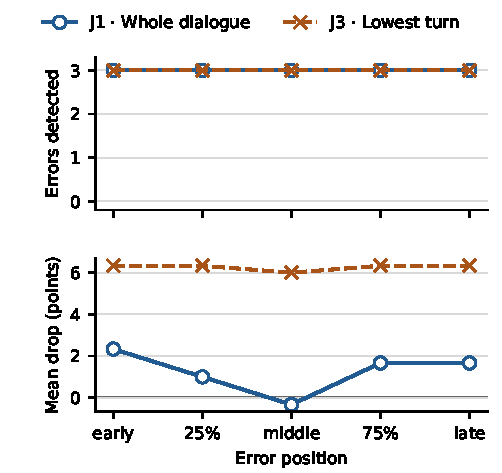
\includegraphics[width=\columnwidth]{position-curve.pdf}
  \caption{Qwen3.5-9B feasibility pilot across five assistant reply positions, with three edited dialogues per position. Detection uses the original pilot labeling rule. Score drops are paired differences from the unedited counterparts on the 1--10 scale.}
  \label{fig:positions}
\end{figure}

\subsection{Correct-route placement controls}

We tested whether the appended sentence could attract criticism even when the route was correct. For each of the 15 route-error variants, we kept the sentence in the same reply and replaced only Ely with the correct requested location. These controls preserve the placement and phrasing of the appended claim. Place names can differ in length. We reran J1 with the same prompt, model and decoding settings on the 15 counterparts using the local model. All 15 returned valid judgments.

We coded a placement flag when the explanation explicitly criticized the appended claim's timing, repetition or relevance. We coded a route challenge when the explanation called the correct location wrong or unsupported. Both tallies are specific to the appended claim and can overlap.

\begin{table}[ht]
  \centering
  \begin{tabular}{lrr}
    \toprule
    Position & Placement flags & Route challenges \\
    \midrule
    Early & 0 & 0 \\
    25\% & 1 & 0 \\
    Middle & 0 & 0 \\
    75\% & 1 & 0 \\
    Late & 2 & 2 \\
    \midrule
    Total & 4 & 2 \\
    \bottomrule
  \end{tabular}
  \caption{J1 flags on the correct-route controls. Each position has three variants. One late route challenge is ambiguous because the explanation also acknowledges the correct destination and ends mid-sentence.}
  \label{tab:route-controls}
\end{table}

J1 flagged placement in four controls, including two closing turns (Table~\ref{tab:route-controls}). In the late Norwich control, J1 correctly recognized that the train task was over and called the requested departure city a hallucination. In the late Peterborough control, J1 called the destination statement incorrect, then acknowledged that the user had requested Peterborough. We count that response as an explicit challenge and treat its rationale as ambiguous.

Relative to these matched correct-route controls, false-route copies scored lower in six pairs, tied in seven, and scored higher in two. The correct-route controls themselves tied the untouched originals in 13 pairs, scored lower in one, and scored higher in one. These comparisons show that J1 can object to the placement of a factual statement and can raise a factual concern about a correct one. With three base dialogues, the controls illustrate the confound and motivate the redesigned pilot.


\section{Changes since the proposal}

The proposal targets 40 base dialogues, five error types, five positions, and five judging setups. We began with one error type and two judging protocols so that we could audit the pipeline and the judgments before scaling. Appending the same route claim at different positions changes its distance from the earlier evidence and its fit with the topic. For example, the Peterborough claim appears immediately before the appended Ely claim in the 25\% variant, while the late variant attaches Ely to a goodbye. Later replies may also appear to repair an earlier mistake. The three base dialogues, conspicuous edits, and saturated detection limit what this pilot can establish about position.

The protocols also differ in the evidence they see and the number of issues they can report. J1 sees later turns and can list three issues in total. J3 flags issues one reply at a time, with the assessed reply always at the end of its input. This design compares the two protocols as complete systems. To test the effect of context access more directly, the follow-up will ask the full-transcript and prefix judges for the same evidence-backed verdict for each reply. Comparing aggregations on the same per-turn scores isolates the effect of the aggregation rule.

\section{Controlled follow-up}

\paragraph{Varying position.}
The next run will use six fresh MultiWOZ-based scenarios, three with a destination constraint and three with a booking-date constraint. Each scenario will have an evidence-and-reply exchange that can move early, to the middle, or late among comparable exchanges. We will keep the chronological window from the constraint to the reply fixed and match the two alternatives at each position. For example, if the user asks to arrive in Peterborough, a confirmation at the target turn can use Peterborough or Ely. Only the confirmed value changes across the two versions. A booking-date item can use the same design with a requested date and a nearby alternative. The three positions and two values produce six variants per scenario, for 36 transcripts.

An exchange can move only when the surrounding turns preserve its meaning in all positions. A later clarification, an explicit change of mind, or a later action that depends on the faulty value may introduce a second detectable issue or change the stakes of the first. We plan to keep cases whose surrounding turns leave the supporting constraint, consequences, and plausibility comparable across positions. We will preserve dialogue length within each scenario where possible and record the exact target index. The main test uses facts established in the transcript. Database-grounded issues would require a separate evidence condition that supplies the same task-relevant records to both protocols.

\paragraph{Validation and readiness.}
Two reviewers will independently check the original constraint, the targeted reply, and the correctly matched version at each position before seeing model scores. They will verify that the incorrect transcript contains one intended violation, that the correct counterpart fulfills the recorded constraint, and that both read naturally. We will document exclusions and adjudicate disagreements using the transcript. Eligibility depends on these checks and is independent of the judge scores on originals. The run will also check that the judge returns a usable verdict for every case. We will proceed to scale when the matched pairs pass review, the primary detector has both hits and misses across scenarios, and it produces at most one targeted false alarm over the 18 correct counterparts.

\paragraph{Outcomes and analysis.}
Each follow-up detection will require the corrupted reply, the specific violated constraint, and a reference to its supporting text. We will retain partial hits separately and report the correct counterpart's score minus its faulty counterpart's score as a signed paired change. For the turnwise judge, we will also report the targeted reply's own score change and which reply set the dialogue minimum. On controls, distinguishing factual false alarms from valid observations about an existing flaw or awkward phrasing helps explain why a score may change.

We will preserve base scenario identifiers and assign distinct identifiers to error families, positions, and correct-or-incorrect variants. All variants of one base scenario remain in the same calibration or evaluation split. We will report detection counts by position with their denominators and select the middle-versus-ends contrast before the larger run. For uncertainty estimates, we will resample base dialogues with all of their paired variants together. The six-scenario result will guide validation and error difficulty. Estimation of position effects and any comparison across additional judge protocols depend on the larger held-out set.

\section{Remaining work}

\begin{itemize}
  \item \textbf{Nov. 21--24.} Prepare and independently verify the matched cases, run the 36-transcript follow-up locally, and check the readiness criteria.
  \item \textbf{Nov. 25--30.} Freeze the labels and selection rules. Expand the dataset as validation allows, prioritizing J1 and J3. Add the constraint rubric, the TD-EVAL adaptation, and the state-tracking judge as compute permits. Compare tracked state with dataset annotations and with state tracking disabled.
  \item \textbf{Dec. 1--8.} Analyze position effects with paired uncertainty, audit representative errors, and reproduce the tables and figures from saved outputs. Present the poster on Dec. 3 and use feedback to revise the final paper and code for Dec. 8.
\end{itemize}

\section*{Acknowledgements}
The proposal disclosed using Claude and Gemini for brainstorming. Codex assisted with code, audit checks, and drafting this milestone.

\clearpage
\bibliography{references}

\end{document}
